\chapter{Mapping} \label{chap:mapping}
For accurate foot placement and localisation purposes the robot makes use of two maps, a sparse map covering a large area, and a dense map covering a small
area around the robot. The primarily use of the sparse map is for localisation and extracting pose data, i.e. orientation, velocity and rate. While the dense
map is used to analyse the terrain and find an appropriate point to place the three supporting feet.
It is possible to also use the sparse map for autonomous navigation, however this use case in not covered in this paper.
This chapter covers the design of the mapping system.

The localisation, sparse mapping and pose estimation is handle by ORB-SLAM3 as described in \cite{campos2021orb}. Since ORB-SLAM3 is not a system designed by the author, its
design will not be covered in this chapter. Implementation and operation details will however be covered in chapters \ref{chap:hardware} and \ref{chap:results}.

\section{Projection}
In order to generate a heightmap from a \ac{rgbd} image, it is first required to project the \ac{rgbd} image into 3D space, this is necessary because a heightmap is essentially a 3D environment,
that can be represented as a image due to the assumption of purely convex geometry. 

The camera can be described by its intrinsic and extrinsic parameters. Extrinsic parameters characterise the
cameras position in 3D space, and intrinsic parameters characterise the relationship between the image plane 3D space, 
assuming the camera is at the world origin and an zero rotation. \cite{hartley2003multiple}.

\newpage
\noindent
Refer to figure \ref{fig:projection} as a visual aid regarding projection. Note that this figure is drawn from the perspective of projecting from the image plane into the world,
if the objective was to project from the world onto the image plane the projection center and image plane would swap places, causing the image to be inverted, thus, this figure assumes
that the image rotation has been corrected.
\begin{figure}[h]
    \centering
    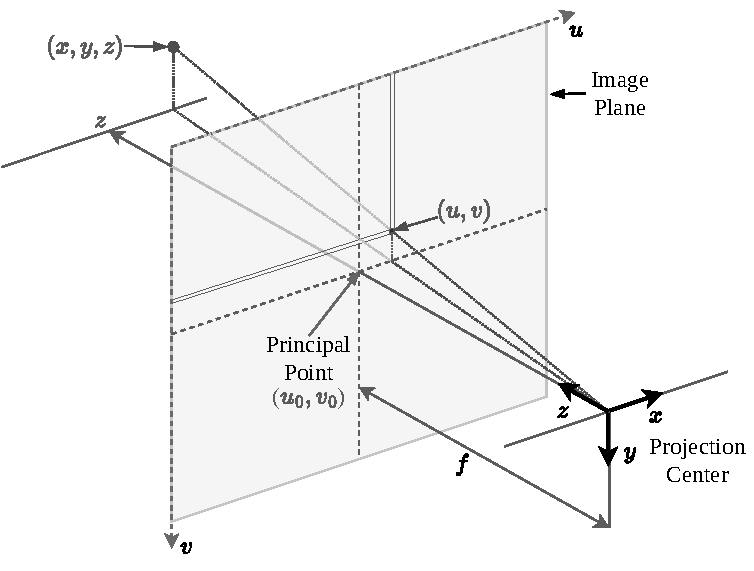
\includegraphics{Diagrams-Projection.drawio.pdf}
    \caption{Camera Projection}
    \label{fig:projection}
\end{figure}

\noindent
Together the extrinsic and intrinsic matrices form the projection matrix,
as shown in equation \ref{eq:projection_matrix},
\begin{equation} \label{eq:projection_matrix}
    \boldsymbol{P} = \boldsymbol{K}
    \begin{bmatrix}
        \boldsymbol{R} & \boldsymbol{T}
    \end{bmatrix}
\end{equation}
where \(\boldsymbol{K}\) is the intrinsic matrix and \(\begin{bmatrix} \boldsymbol{R} & \boldsymbol{T} \end{bmatrix}\) the extrinsic matrix, these are described
in equation \ref{eq:intrinsic} and \ref{eq:extrinsic}.

The projection matrix can be used to project a point on the image plane into world space as shown in equation \ref{eq:full_projection}.

\begin{equation} \label{eq:full_projection}
    \begin{bmatrix}
        u \\
        v \\
        1
    \end{bmatrix}
    = \boldsymbol{P}
    \begin{bmatrix}
        x \\
        y \\
        z \\
        1
    \end{bmatrix}
\end{equation}
where \(u,v\) are the pixel coordinates on the image plane and \(x,y,z\) are the coordinates in world space.
\begin{equation} \label{eq:intrinsic}
    \boldsymbol{K} =
    \begin{bmatrix}
        \alpha_x & \gamma   & u_0 \\
        0        & \alpha_y & v_0 \\
        0        & 0        & 1
    \end{bmatrix}
\end{equation}
where the focal length is represented by,
\[\alpha_x = f \cdot m_y\]
\[\alpha_y = f \cdot m_x\]
with \(m_x\) and \(m_y\) being the inverse of the width and height of a image plane pixel, \(f\) the focal length and \(u_0\),\(v_0\) being the principal point, optimally the center of the image plane.
The skew coefficient, \(\gamma\), is often, and in this case, 0.

The extrinsic matrix is as shown below,
\begin{equation}\label{eq:extrinsic}
    \begin{bmatrix}
        \boldsymbol{R} & \boldsymbol{T}
    \end{bmatrix}
    =
    \begin{bmatrix}
        \boldsymbol{R}_{3\times3} & \boldsymbol{T}_{3\times1} \\
        \boldsymbol{0}_{1\times3} & 1
    \end{bmatrix}
\end{equation}
where \(\boldsymbol{R}\) characterises the camera's heading in world space and \(\boldsymbol{T}\) the world origin expressed in 
the camera coordinate frame.

For ease of preprocessing points are first projected into the camera coordinate frame, in other words, the extrinsic matrix is omitted from equation \ref{eq:full_projection}.
The resultant matrix equation is shown in equation \ref{eq:local_projection}.

\begin{equation} \label{eq:local_projection}
    \begin{bmatrix}
        u \\
        v \\
        1 \\
        1/z
    \end{bmatrix}
    = \frac{1}{z}
    \begin{bmatrix}
        f_x & 0 & c_x & 0 \\
        0 & f_y & c_y & 0 \\
        0 & 0 & 1 & 0 \\
        0 & 0 & 0 & 1
    \end{bmatrix}
    \begin{bmatrix}
        x\\
        y\\
        z\\
        1
    \end{bmatrix}
\end{equation}
From equation \ref{eq:local_projection} \(x,y,z\) are found to be show in equation \ref{eq:proj_z} to \ref{eq:proj_y}.
\begin{align}
    z &= I_{u,v} \label{eq:proj_z}\\[0.2cm]
    x &= \frac{z(u - u_0)}{\alpha_x}\label{eq:proj_x} \\
    y &= \frac{z(v - v_0)}{\alpha_y}\label{eq:proj_y}
\end{align}
where \(I_{u,v}\) is the depth image value at pixel coordinates \(u,v\). For later use \(\boldsymbol{p_{proj}} = [x \; y \; z]\) is defined.

\newpage
\section{Map Buffer}
    Once the depth image is projected into map space, their x and y coordinates are used as indices to write their z value into the heightmap. The heightmap is stored in
    a 2D circular buffer, this means that as the robot moves around, old map data is erased to make room for new data. This structure is illustrated in figure \ref{fig:memory}.
    \begin{figure}[h]
        \centering
        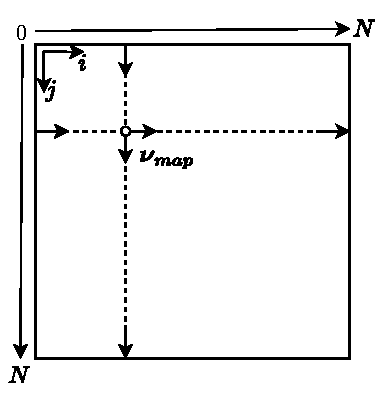
\includegraphics{Diagrams-Memory.drawio.pdf}
        \caption{Memory Diagram}
        \label{fig:memory}
    \end{figure}

    The heightmap buffer, \(\boldsymbol{M}\), is of size \(N \times N\) and is indexed by \(i,j\). The mapping from the projection center relative points, \(\boldsymbol{p_{proj}}\), into map space
    is defined in equation \ref{eq:project_to_map},
    \begin{equation} \label{eq:project_to_map}
        \boldsymbol{p_{map}} = (\boldsymbol{q} \cdot \boldsymbol{p_{proj}} \cdot \boldsymbol{q}^{-1}S + \boldsymbol{\nu_{map}}) \mod N
    \end{equation}
    where \(\boldsymbol{q}\) is the camera quaternion that rotates \(\boldsymbol{p_{proj}}\) into world space, with its \(z\) axis pointing upwards, \(\boldsymbol{\nu_{map}}\) 
    is the coordinate vector of the robot in map space, and \(S\) is the scaling factor
    used to relate heightmap cells to \(cm\). The relationship between \(N, S\) and \(E\) are characterised by equation \ref{eq:map_scaling}.
    \begin{equation} \label{eq:map_scaling}
        N = E \cdot S
    \end{equation}
    where E is the size of the heightmap in \(cm\).

    The robots coordinates in the map space, \(\boldsymbol{\nu_{map}}\), can be found as shown in equation \ref{eq:map_i},
    \begin{equation} \label{eq:map_i}
        \boldsymbol{\nu_{map}} = \boldsymbol{\nu_{world}} \mod N
    \end{equation}
    where \(\boldsymbol{\nu_{world}}\) is the coordinate of the robot in world space.

    \subsection{Between Map and Local Space}
        As the robot commands foot positions in local space, when optimising foot positions (see chapter \ref{chap:optimisation}) it is required to have a translation between map and local space.
        These translations are defined in equation \ref{eq:local_to_map} and \ref{eq:map_to_local_help} to \ref{eq:map_to_local_rot}.
        
        Local to map space is a simple translation, very similar to equation \ref{eq:project_to_map},
        \begin{equation} \label{eq:local_to_map}
            \boldsymbol{\nu_{map}} = (\boldsymbol{q_{bod}} \cdot \boldsymbol{\nu_{loc}} \cdot \boldsymbol{q_{bod}}^{-1} + \boldsymbol{\nu_{map}}) \mod N
        \end{equation}

        However, due to the circular nature of the map buffer, translating from map to local space is more challenging. First an intermediate position, \(\boldsymbol{\nu_{temp}}\) is defined as a helper,
        \begin{equation} \label{eq:map_to_local_help}
            \boldsymbol{\nu_{temp}} = \boldsymbol{\nu_{map}}\frac{1}{S}
        \end{equation}
        now \(\boldsymbol{\nu_{temp}}\) must be checked to see if either of its coordinates exceed half the map extents, if so, then it must be adjusted such that both coordinates fall within \(\frac{1}{2}E\).
        This is expressed in equation \ref{eq:map_to_local_adj}
        \begin{equation} \label{eq:map_to_local_adj}
            \boldsymbol{\nu_{temp}} \Leftarrow 
            \begin{cases}
                \boldsymbol{\nu_{temp}} & \boldsymbol{\nu_{temp}} \leq \frac{1}{2}E \\
                \boldsymbol{\nu_{temp}} - E\sgn \boldsymbol{\nu_{temp}} & \boldsymbol{\nu_{temp}} > \frac{1}{2}E
            \end{cases}
        \end{equation}
        where \(\sgn\) is the signum function, which return either 1 or -1 depending on the sign of the operand. 
        \textbf{Note} that equation \ref{eq:map_to_local_adj} is applied to both coordinates in the vector \(\boldsymbol{\nu_{temp}}\) separately, in pursuit of readability this is not explicitly stated.

        Now that \(\boldsymbol{\nu_{temp}}\) has been corrected for the circular nature of the map buffer, only the rotating into the local space remains.

        \begin{equation} \label{eq:map_to_local_rot}
            \boldsymbol{\nu_{loc}} = \boldsymbol{q_{bod}}^{-1} \cdot \boldsymbol{\nu_{temp}} \cdot \boldsymbol{q_{bod}}
        \end{equation}


